\documentclass{beamer}
\DeclareFontShape{OT1}{cmss}{b}{n}{<->ssub * cmss/bx/n}{} 
\usetheme{default}
\usepackage{amsmath}
\usepackage{amsfonts}
\usepackage{mathbbol}
\usepackage{xcolor} % before tikz or tkz-euclide if necessary
\usepackage{tkz-euclide} % no need to load TikZ
\usepackage{multirow}

\title{Statistical Machine Learning\\ Part 3}
\author{Horacio G\'omez-Acevedo\\ Department of Biomedical Informatics}
\begin{document}
	\begin{frame}[plain]
		\maketitle
	\end{frame}
	\begin{frame}{(Multi)Linear Regression }
		It is very insightful to check the ordinary linear regression as a
		linear algebra problem.
		%
		If we have training data \(\{ (x_1,y_1),\ldots,(x_n,y_n)\}\), let's
		write \(X\) as a \(n\times 2\) matrix 
		\begin{equation*}
		X= \begin{pmatrix}
			\mathbb{1} & \mathbb{X }
		\end{pmatrix}=
		\begin{pmatrix}
			1 & x_1\\
			1 & x_2 \\
		   	\vdots & \vdots \\
			1 & x_n 
		\end{pmatrix}
		\end{equation*} The response variable vector \(Y\), the parameters
		\(\theta_0, \theta_1\) and the vector of random errors are expressed as
		%
		\begin{equation*}
		\mathbb{Y}=
		\begin{pmatrix}
			y_1\\
			y_2\\
			\vdots\\
			y_n
		\end{pmatrix},
		\theta= 
		\begin{pmatrix}
			\theta_0 \\
			\theta_1
		\end{pmatrix}, 
		\varepsilon= 
		\begin{pmatrix}
			\varepsilon_1\\
			\varepsilon_2\\
			\vdots\\
			\varepsilon_n
		\end{pmatrix}
		\end{equation*} 
	\end{frame}

\begin{frame}{(Multi)Linear Regression (cont)}
	Then we can write the population regression formula in a matrix form
\begin{equation}
	\mathbb{Y}=X \cdot \theta + \varepsilon=\theta_0 \mathbb{1}+ \theta_1 \mathbb{X}+ \varepsilon
\end{equation}
The method of least squares reduces to find $(\hat{\theta}_0,\hat{\theta_1})$ that minimizes the function
	\begin{equation*}
		(\theta_0,\theta_1)\mapsto \frac{1}{n}\sum_{i=1}^n (y_i- \theta_0-\theta_1 x_i)^2
	\end{equation*}
\end{frame}

\begin{frame}{Least Squares Function}
	As we can see in the following graph, the projection of the minimum value will be the estimates of $\hat{\theta}_0$ and $\hat{\theta}_1$.
	\begin{figure}[h]
		\centering
		\includegraphics[scale=0.5]{../../Figures/fig_minfunc.png}
	\end{figure}
\end{frame}
	
\begin{frame}{Multidimensional Interpretation}
If we plot the vectors $\mathbb{1}$ and $\mathbb{X}$, the hyperplane (generated) by those vectors, contains a vector $\mathbb{V}$ which is closest to the vector $\mathbb{Y}$.  It can be proven that the vector $\mathbb{V}$ can be written as
\begin{equation*}
	\mathbb{V} = X (X^t X)^{-1} X^t \mathbb{Y}
\end{equation*}
On the other hand 
\begin{equation*}
	\mathbb{V}= X \cdot \begin{pmatrix} \hat{\theta}_0\\ \hat{\theta}_1 \end{pmatrix}
\end{equation*}
Thus
\begin{equation}
	\begin{pmatrix}
		\hat{\theta}_0\\ \hat{\theta}_1
\end{pmatrix} = (X^t X)^{-1} X^t \mathbb{Y}
\label{eq:normeq}
\end{equation}	
This last equation is called the {\bf normal form}
\end{frame}

\begin{frame}{Multidimensional Interpretation}
	
	\begin{figure}[h]
		\centering
		\includegraphics[scale=0.5]{../../Figures/fig_projection.png}
	\end{figure}
\end{frame}

\begin{frame}{Computational Complexity}
	The solution of the linear regression problem using the normal equation (\ref{eq:normeq}), requires significant amount of computation resources as $n$ tend to increase.
	
	Let $f,g \colon \mathbb{N} \to \mathbb{R}^+$ two non-negative functions. We say that $f(n)= O(g(n))$ (big O) if there are two non-negative integers $n_0$ and $c$ such that for every $n\ge n_0$
	\begin{equation*}
		f(n) \le c \cdot  g(n)
	\end{equation*}
  {\bf Example.} Let $f(n)=5n^3+3n^2+1000n +10000$. In this case $f(n)=O(n^3)$ since when $n$ is very large, $f(n)$ behaves like the polynomial $5n^3$.
  
  The complexity of matrix inversion is between $O(n^{2.4})$ and $O(n^3)$, depending on the algorithm.
\end{frame}			

\begin{frame}{Gradient Descent Revisited}
	
	In a previous lecture, we have defined the general gradient descent rational as reaching the (hopefully global) minimum iteratively using a formula like 
	\begin{equation*}
		\theta^{k+1}= \theta^k - \eta(k) \nabla J(\theta^k)
	\end{equation*}
	In the context of linear regression, $J(\mathbf{x})= MSE(\mathbf{x})$. Since the $MSE$ is a convex function, a global minimum can be reached! Thus after a certain number of steps $m$ we say that $\theta^m$ is (close enough) to the linear regression problem 
	\begin{equation*}
	 {X}  \cdot \theta ^m \approx \mathbb{Y}
	\end{equation*}

{\bf Note.} In G\'eron's book the notation is just a bit different (by using the transpose), but the concepts are totally equivalent.
\begin{equation*}
	MSE(\theta)=  \frac{1}{m} \sum_{i=1}^m (\theta^T \cdot \mathbf{x}^{(i)} - y^{(i)})^2
\end{equation*}
\end{frame}
\begin{frame}{Stochastic Gradient Descent}
	For the {\bf cost function} MSE, the gradient is calculated as
	\begin{equation*}
		\nabla_\theta MSE (\theta)= \frac{2}{m} X^t (X \cdot \theta)-\mathbb{Y}
	\end{equation*}
Thus, at each step of the gradient descent, we need to recalculate the gradient using the whole dataset. This operation is expensive as matrix multiplication continue to pile up. One solution is to use the calculations of the gradient taking instances in the training set at every step and computing  gradients based only on that instance. 


\end{frame}

\begin{frame}{Regularized Linear Models (Shrinkage)}
Traditionally these methods involves using least squares to fit a linear model that contains a subset of the predictors (ergo the name shrinkage).  These techniques {\it constrains} or {\it regularizes} the coefficient estimates towards zero.

\begin{equation*}
	RSS= \sum_{i=1}^n \left( y_i - \theta_0 - \sum_{j=1}^p \theta_j x_{ij} \right)^2
\end{equation*}

In {\bf ridge regression}, the coefficients are estimated by minimizing a slightly different quantity. The ridge regression coefficient estimates $\hat{\theta}^R$ that minimize
\begin{equation*}
\sum_{i=1}^n \left( y_i - \theta_0 - \sum_{j=1}^p \theta_j x_{ij} \right)^2 + \lambda \sum_{j=1}^p \theta_j^2,
\end{equation*} 
where $\lambda \ge 0$ is a tuning parameter (hyperparameter) to be determined separately. 




\end{frame}

\begin{frame}{Ridge Regression (cont)}
	
	The shrinkage penalty is applies to $\theta_1,\ldots, \theta_p$ but not to intercept $\theta_0$.  Since this is the measure of the mean value of the response when $x_{i1}=x_{i2}=\cdots=x_{ip}=0$.
	
	One of the main reasons to use ridge regression is in the bias-variance trade-off. As $\lambda $ increases, the flexibility of the ridge regression fit decreases leading to decreased variance but increased bias. 
	
	One disadvantage of ridge regression is that it will include all $p$ predictors in the final model. The penalty term $\lambda \sum_{i=1}^p \theta_j$ will shrink all the coefficients towards zero, but it will not set any of them exactly to zero. 
\end{frame}

\begin{frame}{Lasso}
	The {\bf Lasso} alternative calculates the coeffcients $\hat{\theta}_\lambda^L$ by minimizing a slightly different formula
\begin{equation*}
	\sum_{i=1}^n \left( y_i - \theta_0 - \sum_{j=1}^p \theta_j x_{ij} \right)^2 + \lambda \sum_{j=1}^p |\theta_j|,
\end{equation*} 	
	The advantage of lasso is that it forces some of the coefficien estimates to be exactly equal to zero when the tuning parameter $\lambda$ is sufficiently large. Thus, we say that lasso yields {\it sparse} models.
\end{frame}

\begin{frame}{Optimization perspective}
	Ridge regression can be seen as the minimization of the following problem
	\begin{equation*}
		\min_{\theta} \left\{ \sum_{i=1}^n \left( y_i - \theta_0 - \sum_{j=1}^p \theta_j x_{ij} \right)^2 \right\} \quad\textrm{subject to }   \sum_{j=1}^p \theta_j^2 \le s
	\end{equation*} 
whereas the lasso becomes 
\begin{equation*}
	\min_{\theta} \left\{ \sum_{i=1}^n \left( y_i - \theta_0 - \sum_{j=1}^p \theta_j x_{ij} \right)^2 \right\} \quad\textrm{subject to }   \sum_{j=1}^p |\theta_j | \le s
\end{equation*} 

\end{frame}

\begin{frame}{Optimization picture}
	The ellipses that are centered around $\hat{\theta}$ represent regions of constant RSS. The intersections between the lasso and ridge regression coefficient estimates with the ellipses. Notice that for the lasso the point of contact has $\theta_1=0$, whereas for the ridge regression the value of $\theta_1$ is "small" but does not vanish.
		\begin{figure}[h]
		\centering
		\includegraphics[scale=0.5]{../../Figures/fig_lasso_ridge.png}
	\end{figure}
	
\end{frame}

\begin{frame}{Problem with Lasso}
For Lasso Regression the cost function is defined as
\begin{equation*}
	J(\theta)=MSE(\theta)+\alpha\sum_{i=1}^n |\theta_i|
\end{equation*}
However, the absolute function is not differentiable at zero! So, we use the right or left hand derivatives. More precisely,

\begin{equation*}
	g(\theta,J)= \nabla_\theta MSE (\theta)+ \lambda  
	\begin{pmatrix}
		\textrm{sign}(\theta_1)\\
		\vdots\\
		\textrm{sign}(\theta_n)
	\end{pmatrix}
\end{equation*}
where 
\begin{equation*}
	\textrm{sign}(x)= \begin{cases}
		1 & \textrm{if } x>0\\
		0 & \textrm{if } x=0\\
		-1 & \textrm{if  }x<0
	\end{cases}
\end{equation*}
\end{frame}

\begin{frame}{Elastic Network}
This model is a (convex) combination between Ridge Regression and Lasso Regression. For $r \in [0,1]$ and $s \ge 0$ the optimization goal is

\begin{equation*}
	\begin{split}
\min_{\theta} \left\{ \sum_{i=1}^n \left( y_i - \theta_0 - \sum_{j=1}^p \theta_j x_{ij} \right)^2 \right\}  \\
\quad\textrm{subject to }   (1-r)\sum_{j=1}^p |\theta_j | + r \sum_{j=1}^p \theta_j^2 \le s
	\end{split}
\end{equation*} 

\end{frame}


\begin{frame}{References}
	
	Materials and some of the pictures are from (1),(2), and (3).
	\begin{enumerate}
		\item Gareth James et al. {\it An Introduction to Statistical Learning with applications in R}. Springer (2015)
		\item Richard O. Duda et al. {\it Pattern Classification} John Wiley (2001). 
		\item Aur\'elien G\'eron. {\it Hands-on Machine Learning with Scikit-Learn \& TensorFlow} O'Relly (2017)
		\item Wiebe R. Pestman {\it Mathematical Statistics} de Gruyter (1998)
	\end{enumerate}	
	
	I have used some of the graphs by hacking TiKz code from StakExchange, Inkscape for more aesthetic plots and other old tricks of \TeX
\end{frame}		
\end{document}


%\subsection{Matrix Form of OLR}\label{matrix-form-of-olr}}
%
%{\it Algebra is generous; she often gives more than is asked of her.}\\
%{\bf Jean le Rond d'Alembert}
%
%
%It is very insightful to check the ordinary linear regression as a
%linear algebra problem.
%
%If we have training data \(\{ (x_1,y_1),\ldots,(x_n,y_n)\}\), let's
%write \(X\) as a \(n\times 2\) matrix \begin{equation}
%X= 
%\begin{pmatrix}
%	1 & x_1\\
%	1 & x_2 \\
%	\vdots & \vdots \\
%	1 & x_n 
%\end{pmatrix}
%\end{equation} The response variable vector \(Y\), the parameters
%\(\theta_0, \theta_1\) and the vector of random errors are expressed as
%
%\begin{equation}
%Y=
%\begin{pmatrix}
%	y_1\\
%	y_2\\
%	\vdots\\
%	y_n
%\end{pmatrix},
%\theta= 
%\begin{pmatrix}
%	\theta_0 \\
%	\theta_1
%\end{pmatrix}, 
%\varepsilon= 
%\begin{pmatrix}
%	\varepsilon_1\\
%	\varepsilon_2\\
%	\vdots\\
%	\varepsilon_n
%\end{pmatrix}
%\end{equation} Then we can write the population regression formula in a matrix form
%\begin{equation}
%Y=X \cdot \theta + \varepsilon
%\end{equation}
%
%During least squared method it is shown that the so-called
%\textbf{normal equations} are satisfied by the estimates of
%\(\hat{\theta}\)
%
%\begin{equation}
%\begin{split}
%	n \hat{\theta}_0 + \hat{\theta}_1 \sum x_i &= \sum y_i\\
%	\hat{\theta}_0 \sum x_i + \hat{\theta}_1 \sum x_i^2  &= \sum x_iy_i
%\end{split}
%\Rightarrow X^t \cdot X \cdot \hat{\theta}= X^t \cdot Y
%\label{eq:hat1}
%\end{equation} where \begin{equation}
%X^t\cdot X = 
%\begin{pmatrix}
%	n & \sum x_i\\
%	\sum x_i & \sum x_i^2
%\end{pmatrix}
%\end{equation}
%
%It can be shown that \begin{equation*}
%\det (X^t\cdot X) = n \sum (x_i - \overline{x})^2 >0
%\end{equation*} (except in the trivial case where all the \(x_i\)'s
%are the same). Thus, the matrix is invertible. Then, from equation
%(\ref{eq:hat1}) we have
%
%\begin{equation}
%\hat{\theta}= 
%\begin{pmatrix}
%	\hat{\theta}_0 \\
%	\hat{\theta}_1 \\
%\end{pmatrix} = (X^t \cdot X)^{-1} X^t \cdot Y
%\end{equation}
%
%From here, we use the following simple observation \begin{equation}
%\hat{Y}= X \cdot \hat{\theta}\Rightarrow \hat{Y}= X\cdot(X^t \cdot X)^{-1} \cdot X^t \cdot Y
%= H \cdot Y
%\end{equation} where the matrix \(H\) is called the \textbf{hat matrix}.
%
%The hat matrix is idempotent i.e. \(H^2=H\).
%
%As for the vector of residuals, \begin{equation}
%\mathbf{e}= Y-\hat{Y} = Y- X \cdot \hat{\theta}= Y-HY= (I_n-H)Y
%\end{equation}
%
%In the setup for linear regression, the variance-covariance matrix of
%the residuals
%
%\begin{equation}
%\sigma^2(\mathbf{e}) = \sigma^2 (I_n -H)
%\end{equation}
%
%Note that \(X \cdot \hat{\theta}\) is the vector of the expected values
%of the \(y_i\) observations. Thus we can write \begin{equation}
%E(Y)=X \cdot \hat{\theta}
%\end{equation} From the computational point of view, instead of solving
%constantly an optimization problem, we can quickly calculate parts of
%the hat matrix.\\
%\begin{equation*}
%(X^t \cdot X)^{-1} = 
%\begin{pmatrix}
%	\frac{1}{n} + \frac{ \overline{x}^2}{\sum (x_i-\overline{x})^2} &
%	\frac{-\overline{x}}{\sum (x_i-\overline{x})^2} \\
%	\frac{-\overline{x}}{\sum (x_i-\overline{x})^2} &
%	\frac{1}{\sum (x_i-\overline{x})^2}
%\end{pmatrix}
%\end{equation*}
%
%A good reference for statistics is the extensive book of Kutner et. al.
%\emph{Applied Linear Statistical Models} with its close to 1400 pages
%but unfortunately no R code (as far as I know).
